\section{Calculating the Water Cross Section}
\label{sec:xsec}

In Section \ref{sec:selection}, highly pure samples of $\nu_\mu$ induced charged
current inclusive events were selected during water-in and water-out running
periods of the P0D. In this section, a cross
section on water is extracted by a direct subtraction of data
from water-in and water-out configurations. We use the MC
simulation to predict the background contamination in the sample and to evaluate the selection efficiency. While the flux distributions used later in this Section were taken from work done by the T2K beam group, the remainder of the cross section extraction was completed by us.

\subsection{Derivation of Statistical Subtraction Formula}

A general cross section $\sigma$~(cm$^2$/nucleon) is related to the true event rate as
follows:

\begin{equation}
N^{true} = \sigma T \Phi
\label{eqn:xsec1}
\end{equation}

where $N^{true}$ is the number of neutrino induced interactions
occurring in a volume containing $T$ total nucleons (neutrons and protons) with
a neutrino flux of $\Phi$~(cm$^{-2}$). If we know the background rate ($B$)
and efficiency ($\epsilon$) of a particular selection, then $N^{true}$ can also be
related to $N^{obs}$, the observed number of interactions:

\begin{equation}
N^{true}=\frac{N^{obs}-B}{\epsilon}.
\label{eqn:xsec2}
\end{equation}

Putting together equations \ref{eqn:xsec1} and \ref{eqn:xsec2}, we get
the general cross section formula:

\begin{equation}
\sigma = \frac{N^{obs}-B}{\epsilon \Phi T}.
\label{eqn:xsec3}
\end{equation}

We extend this simple formulation to the multi-sample, multi-target
case in the P0D. There are two types of data, water-in and water-out(air), as
well as many types of target material in the P0D. Using two versions of
equation \ref{eqn:xsec1}, we get
\begin{eqnarray}
N^{true}_1 &=& \Phi_1 \sigma_w T_w + \Phi_1 \sum\limits_{i}\sigma_i
T_i \nonumber \\
N^{true}_2 &=& \Phi_2 \sum\limits_{i}\sigma_i T_i + \Phi_2 \sigma_{air} T_{air}\nonumber
\label{eqn:xsec4}
\end{eqnarray}
\noindent where $N_1$ and $N_2$ are the total neutrino interactions in water-in
and water-out data, respectively. The cross section on air ($\sigma_{air}$) and the number of air nucleons ($T_{air}$) are both very small, so the second term in the $N^{true}_2$ equation is neglected. Since the water-in configuration of the P0D
has water and includes various other target materials, we sum up the
contributions individually. The $\Phi_1 \sigma_w T_w$ yields the
water-only contribution to the interaction rate and the $\Phi_1
\sum\limits_{i}\sigma_i$ term yields the contribution from all other
target materials summed over material type $i$. The water-out configuration
of the P0D has the exact same material types as the water-in
configuration except for air instead of water. So other than a different flux term
($\Phi_2$), the water-out equation looks similar to the water-in
equation. As we are interested in the water cross section, we solve
for $\sigma_w$, which together with equation \ref{eqn:xsec2} yields:

\begin{equation}
\sigma_w = \frac{1}{T_w}\left[\frac{N^{obs}_1-B_1}{\epsilon_1
    \Phi_1}-\frac{N^{obs}_2-B_2}{\epsilon_2\Phi_2}\right].
\label{eqn:xsec5}
\end{equation}

MC estimations of $B_1$, $B_2$, $\epsilon_1$ and $\epsilon_2$
in conjunction with the water-in and water-out selections from data then
allow us to extract the water cross section. There are a few additional considerations. As seen in Figures \ref{fig:xsZw} and \ref{fig:xsZa}, the selected number of events $N^{obs}_1$ and $N^{obs}_2$, the background terms $B_1$ and $B_2$ and the efficiency terms $\epsilon_1$ and $\epsilon_2$ are all dependent on the beam run number and the Z position of the interaction vertex. The flux terms $\Phi_1$ and $\Phi_2$ are dependent on the beam run number as the beam luminosity increased over the course of the experiment. Therefore, we rewrite the cross section equation as follows:

\begin{equation}
\sigma_w = \frac{1}{T_w}\left[\frac{1}{\sum\limits_r \Phi_1(r)}\sum\limits_{r}^{1,2,4} \sum\limits_{z}^{40} \frac{N^{obs}_1(r,z)-B_1(r,z)}{\epsilon_1(r,z)}-\frac{1}{\sum\limits_r \Phi_2(r)}\sum\limits_{r}^{2,3,4} \sum\limits_{z}^{40} \frac{N^{obs}_2(r,z)-B_2(r,z)}{\epsilon_2(r,z)}\right].
\label{eqn:xsec6}
\end{equation}

Here the Z position of the vertex is assumed to be binned according to p0dule number in the P0D. This is sensible as the expected vertex resolution in the z direction is 1 p0dule. The summation indices ``r" and ``z" correspond with beam run number and p0dule number respectively.

\subsection{Evaluating the Efficiency and Background}

An identical selection applied to the Monte Carlo simulation of P0D
data allows us to extract estimates of the selection efficiency and
backgrounds in water-in runs 1, 2 and 4 and water-out runs 2, 3 and 4. These estimates are used to correct the measured event rates in data and extract the true number of signal events in the water target. Our signal is defined as true $\nu_\mu$ induced charged
current interactions within the fiducial volume of the P0D. The backgrounds are defined as any interaction that (1) is induced by $\overline{\nu_\mu}$,
$\nu_e$, or $\overline{\nu_e}$, (2) occurs outside the fiducial volume or (3)
is non-CC. These three backgrounds are plotted as a function of P0Dule \# in Figures \ref{fig:xsbgrunw} to \ref{fig:xsbgruna}.

\begin{figure}[h]
\centering
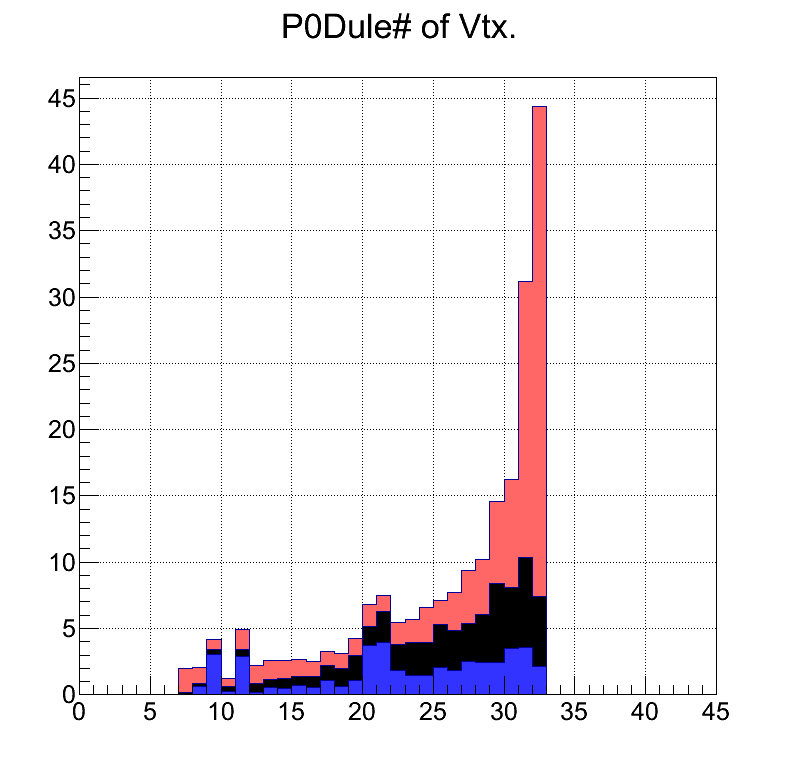
\includegraphics[width=2in]{Figures/TN100Plots/cBG1w.png}
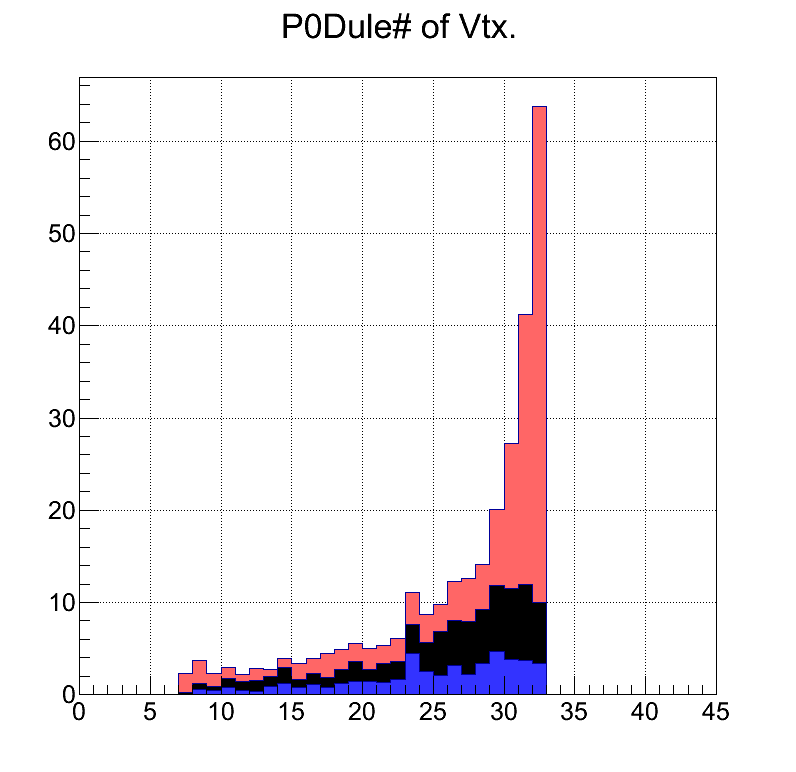
\includegraphics[width=2in]{Figures/TN100Plots/cBG2w.png}
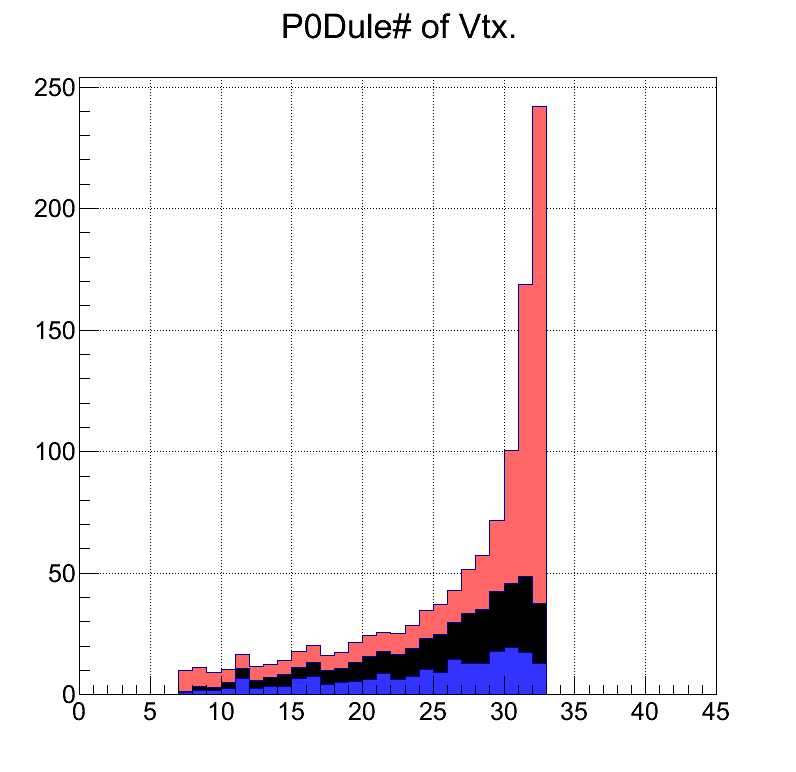
\includegraphics[width=2in]{Figures/TN100Plots/cBG4w.png}
\caption{The selected background as predicted by MC and divided into three background types for run 1 water-in, run 2 water-in and run 4 water-in (left to right). The three background types are out-of-fiducial-volume (red), non-CC (black) and non-$\nu_\mu$ (blue).}
\label{fig:xsbgrunw}
\end{figure}

\begin{figure}[h]
\centering
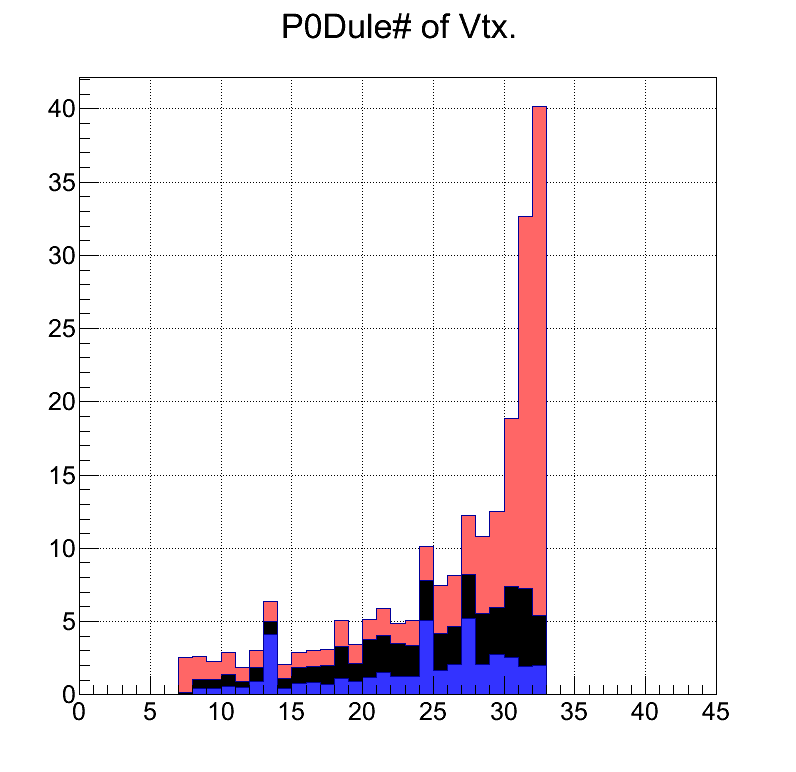
\includegraphics[width=2.5in]{Figures/TN100Plots/cBG2a.png}
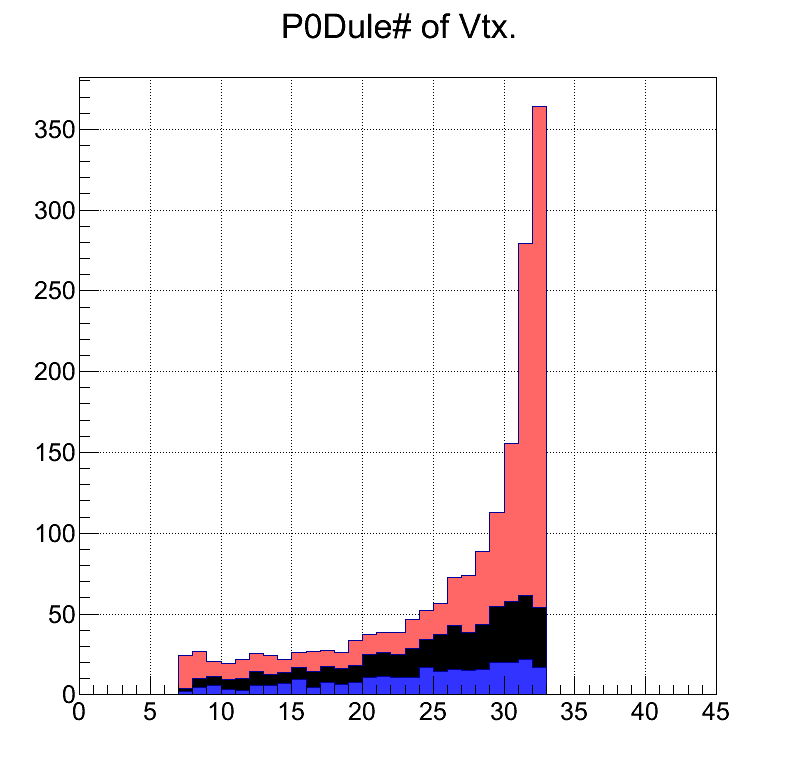
\includegraphics[width=2.5in]{Figures/TN100Plots/cBG3a.png}
\caption{The selected background as predicted by MC and divided into three background types for run 2 water-out and run 3 water-out. Note that run 4 uses the same MC files as run 3 water-out and is therefore not shown. The three background types are out-of-fiducial-volume (red), non-CC (black) and non-$\nu_\mu$ (blue).}
\label{fig:xsbgruna}
\end{figure}

\begin{figure}[h]
\centering
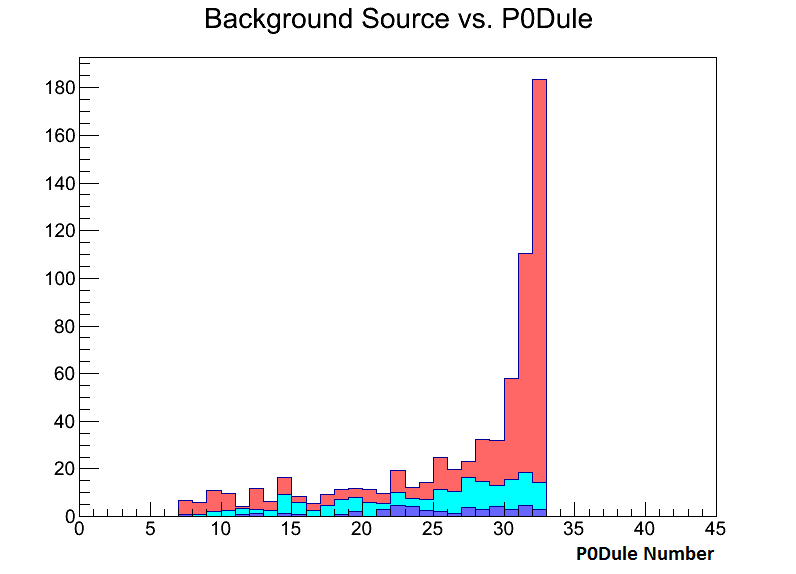
\includegraphics[width=3in]{Figures/BGw.png}
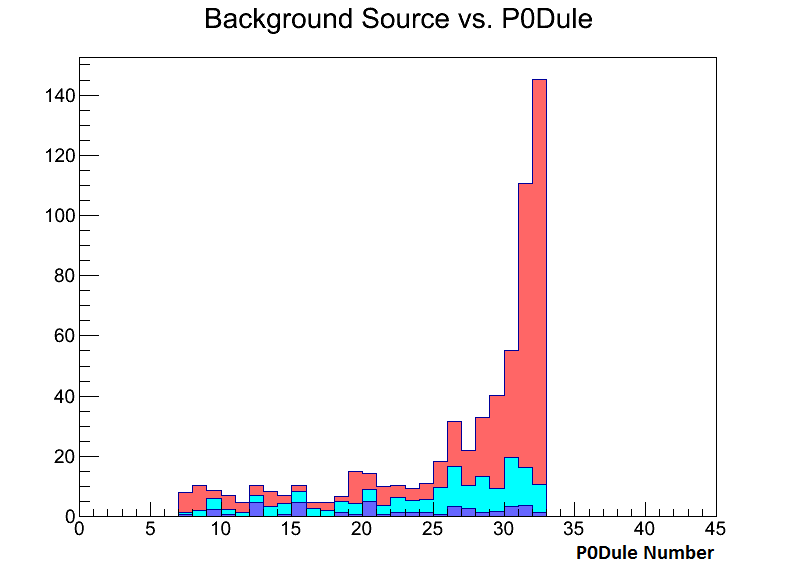
\includegraphics[width=3in]{Figures/BGa.png}
\caption{The selected background as predicted by MC and divided into three background types when integrated over all runs. The three background types are out-of-fiducial-volume (red), non-CC (cyan) and non-$\nu_\mu$ (dark blue). Water-in MC is to the left and water-out MC is to the right.}
\label{fig:xsbg}
\end{figure}

Figure \ref{fig:xsbg} shows the amount of background contamination as predicted by MC for water-in and water-out periods. It is separated into the three types of background types. As expected, we have a highly pure sample. The majority of the background comes from events occuring downstream of the water-target and having a vertex reconstructed inside the fiducial volume. The contribution from non-CC, non-$\nu_\mu$ and sideways entering out-of-fiducial events is extremely small. The reason we have a higher out-of-fiducial-volume (OOFV) background in the downstream end is simply because backwards going tracks do not penetrate very far into the fiducial volume. So the probability of having an event originating from downstream of the fiducial volume and having a reconstructed vertex inside the fiducial volume drops off very quickly as we move away from the downstream edge. Also, given that the selection chooses primarily forward-going muon tracks and the vertex resolution in the XY plane, contamination from OOFV background is low at the sides of the fiducial volume.

Figures \ref{fig:xsZw} and \ref{fig:xsZa} show the behavior of the selection efficiency as predicted by MC. The efficiency varies mostly due to an angular and momentum acceptance effect. We only select events that have a muon that enters the TPC downstream of the P0D. The allowed solid angle for tracks is significantly greater in the downstream region of the P0D than the upstream region. Also, the allowed range of muon momentum is greater in the downstream region of the P0D than the upstream region due to energy loss. The combination of these two effects yields a selection efficiency that varies as a function of the Z position of the interaction vertex.

As efficiency and background are both predominantly functions of the Z vertex position, we apply the efficiency correction and background subtraction also as a function of Z (see eqn. \ref{eqn:xsec6}). The reconstruction vertex resolution in Z is nominally 1 p0dule, so the selected number of events in data for each p0dule is background subtracted and efficiency corrected individually. Also, as the runs have different detector setup, beam power, etc., we also calculate the MC predicted background and signal efficiency separately for each run type and number. The end result is summed together over p0dule number, run type and run number to calculate the total true observed signal interactions in the water-target fiducial volume. The background-subtracted and efficiency-corrected ((N-B)/$\epsilon$) distributions are shown in Figure \ref{fig:xstot} for water-in and water-out. The data and MC shapes agree quite well though there is an overall normalization difference of about $15\%$. The bin contents of these 2D plots are the exact values used in Formula \ref{eqn:xsec6} for the $B_1(r,z)$, $B_2(r,z)$, $\epsilon_1(r,z)$ and $\epsilon_2(r,z)$ terms. Here the subscripts 1 and 2 correspond to water-in and water-out run types respectively. Finally, the integrated results are summarized in Table \ref{tab:xscalc}. The total MC background and signal efficiency as a function of p0dule \# for each run type and run \# is shown in Figures \ref{fig:xsBGvZ} and \ref{fig:xseffvZ}.

\begin{figure}[h]
\centering
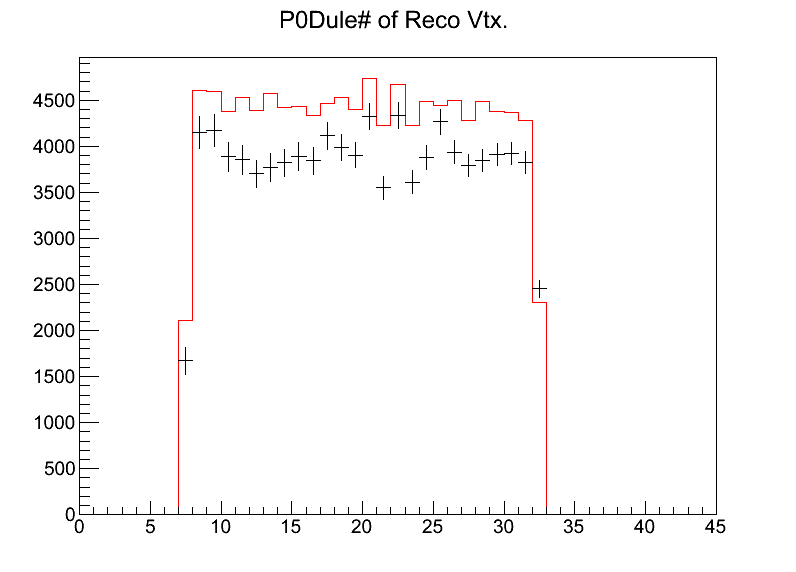
\includegraphics[width=3in]{Figures/TN100Plots/cNBEw.png}
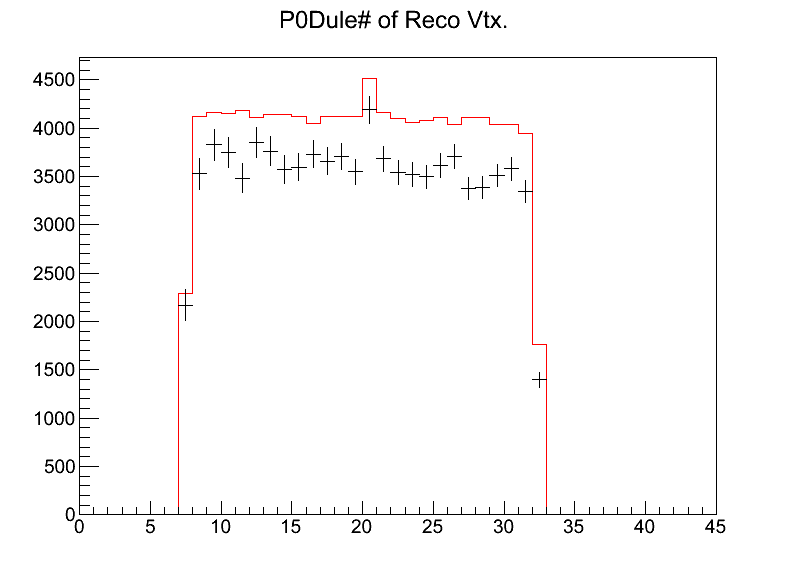
\includegraphics[width=3in]{Figures/TN100Plots/cNBEa.png}
\caption{The total signal binned by p0dule number for water-in runs (left) and water-out runs (right). The black crosses shows the expected signal calculated using the selected event rate in data and the MC for background and efficiency estimates. The red shows the signal according to the MC.}
\label{fig:xstot}
\end{figure}

\begin{figure}[h]
\centering
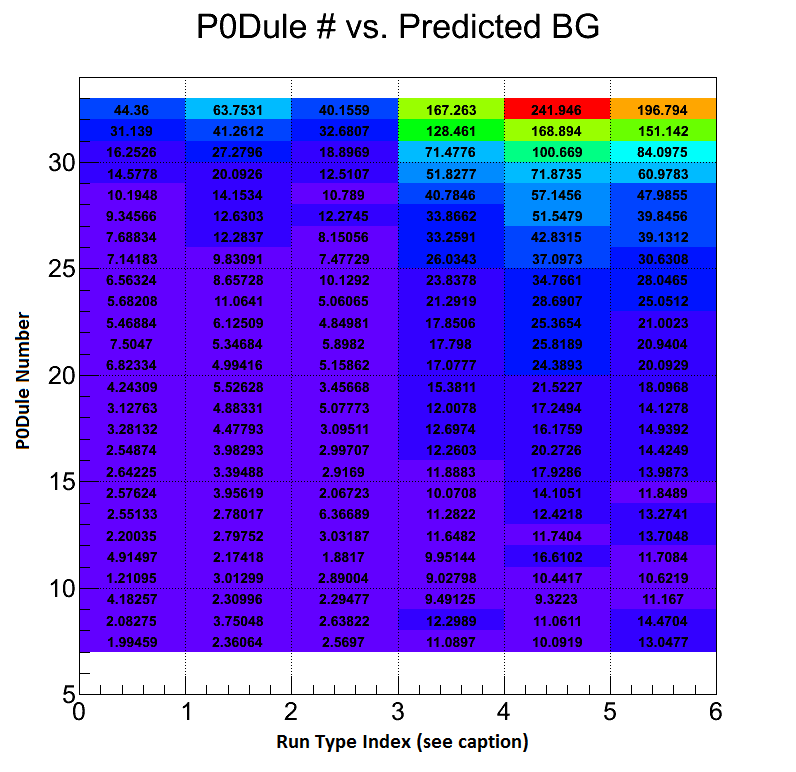
\includegraphics[width=6in]{Figures/TN100Plots/cBG_RvZ.png}
\caption{The total predicted background from MC binned by p0dule number (y-axis) and run number/type (x-axis) for all runs. The x-axis index corresponds to run 1 water-in, run 2 water-in, run 2 water-out, run 3 water-out, run 4 water-in and run 4 water-out from left to right.}
\label{fig:xsBGvZ}
\end{figure}

\clearpage

\begin{figure}[h]
\centering
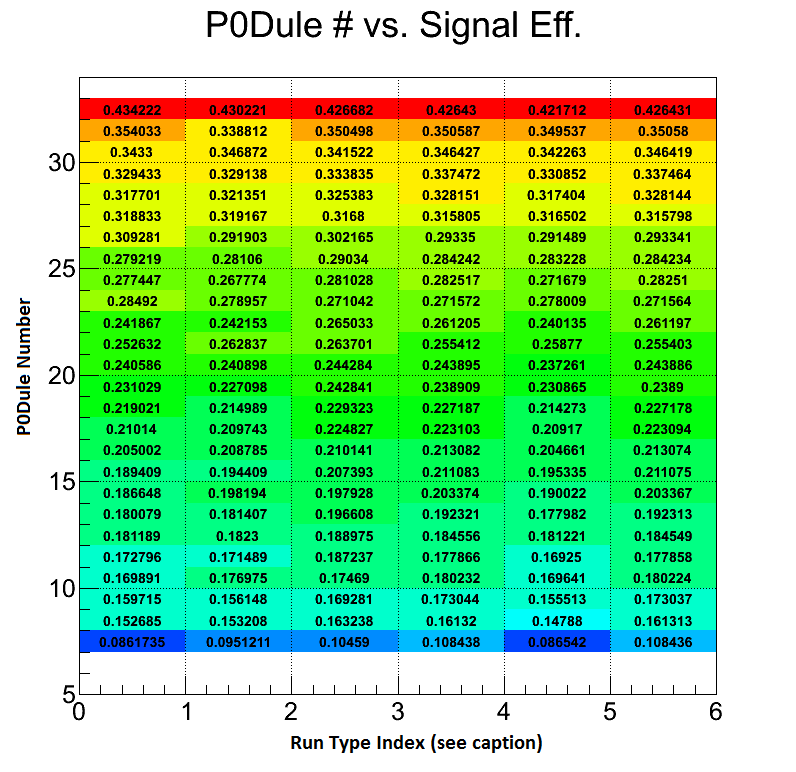
\includegraphics[width=6in]{Figures/TN100Plots/cEff_RvZ.png}
\caption{The signal efficiency from MC binned by p0dule number (y-axis) and run number/type (x-axis) for all runs. The x-axis index corresponds to run 1 water-in, run 2 water-in, run 2 water-out, run 3 water-out, run 4 water-in and run 4 water-out from left to right.}
\label{fig:xseffvZ}
\end{figure}

\clearpage

\subsection{Calculating the Flux Normalization}

We calculate the total flux from the relevant flux distributions for each beam run period. The flux is integrated up to a neutrino energy of 20~GeV and then multiplied by the integrated POT corresponding to each run period. We then sum the total neutrino flux over all the run periods. Figure \ref{fig:fluxes} shows the flux distributions used for each run period.

We are not as efficient at reconstructing and selecting events generated by lower ($<1$~GeV) energy neutrinos as we are for higher energy neutrinos. This is included in the selection efficiency ($\epsilon$) as a function of P0Dule number that we use in our cross section formula. For clarity, we have included plots of the true neutrino energy distributions of the selected MC events in different runs and more importantly, the efficiency as a function of neutrino energy (Figure \ref{fig:nuEeff}).

\begin{figure}[h]
\centering
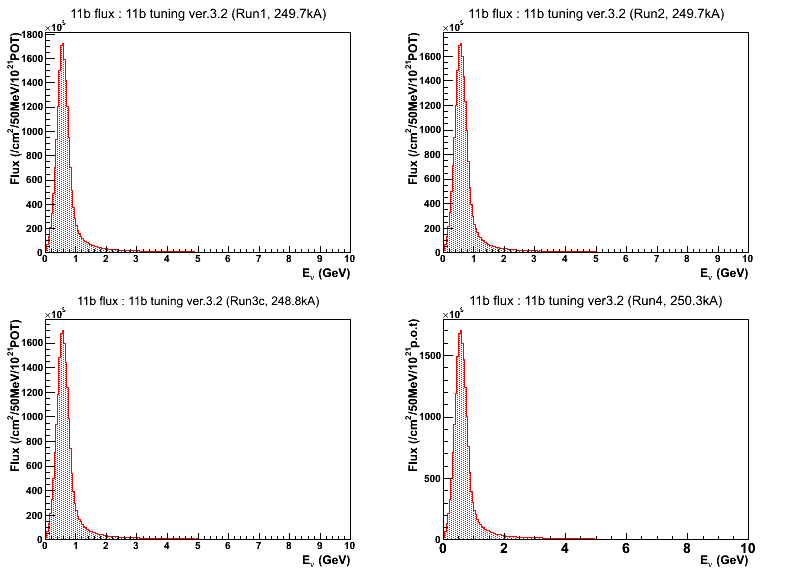
\includegraphics[width=5in]{Figures/fluxes.png}
\caption{The different flux distributions for each run.}
\label{fig:fluxes}
\end{figure}

\begin{figure}[h]
\centering
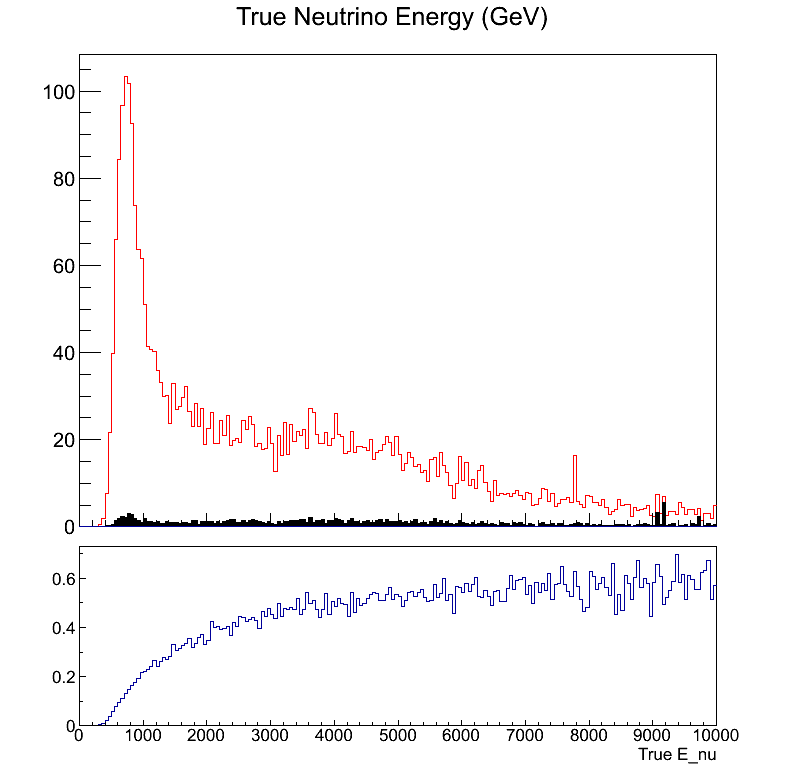
\includegraphics[width=2.5in]{Figures/TN100Plots/c_nuEwater_1.png}
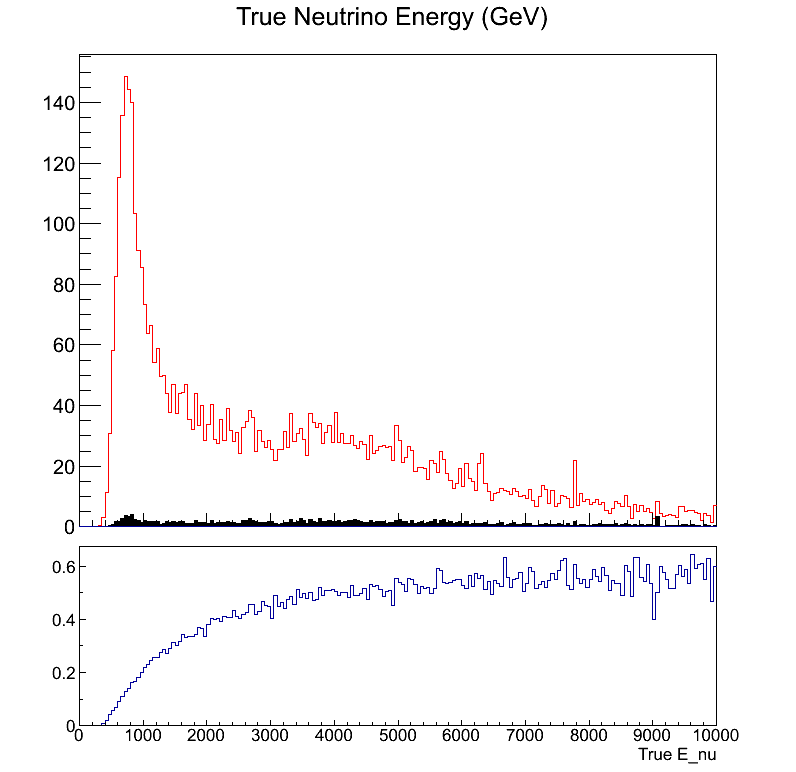
\includegraphics[width=2.5in]{Figures/TN100Plots/c_nuEwater_2.png}
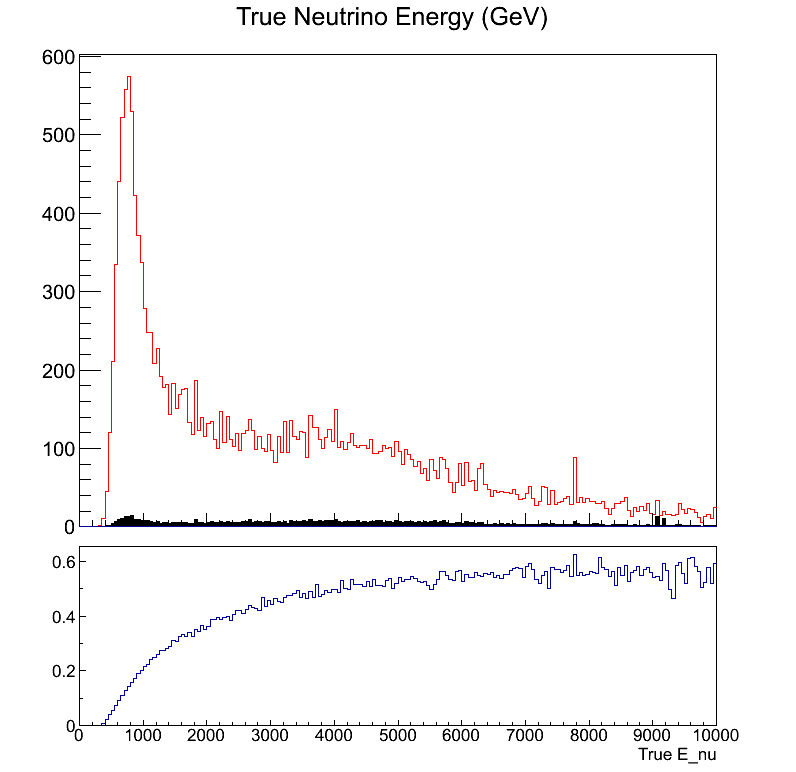
\includegraphics[width=2.5in]{Figures/TN100Plots/c_nuEwater_4.png}
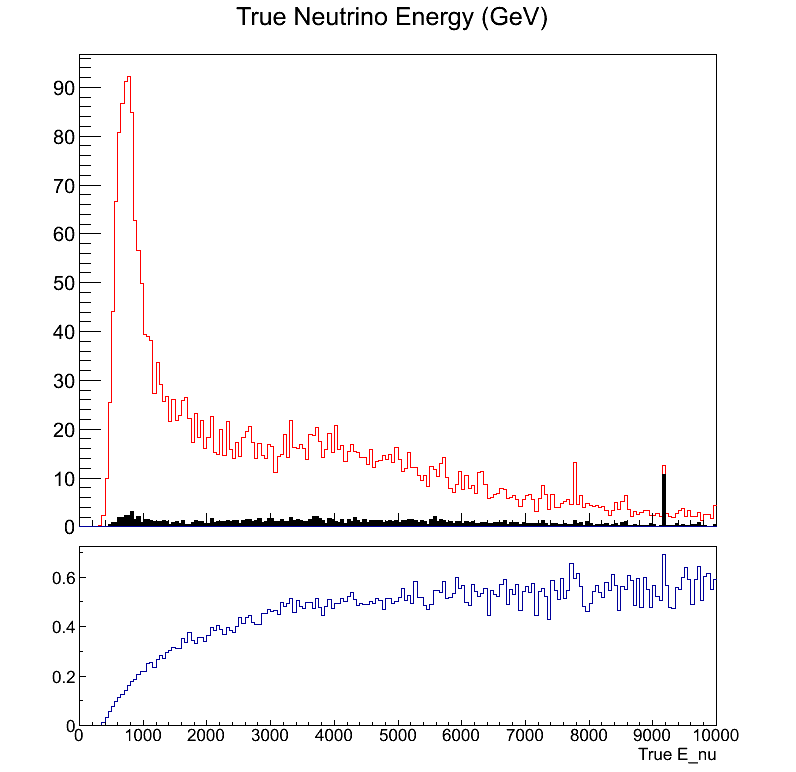
\includegraphics[width=2.5in]{Figures/TN100Plots/c_nuEair_2.png}
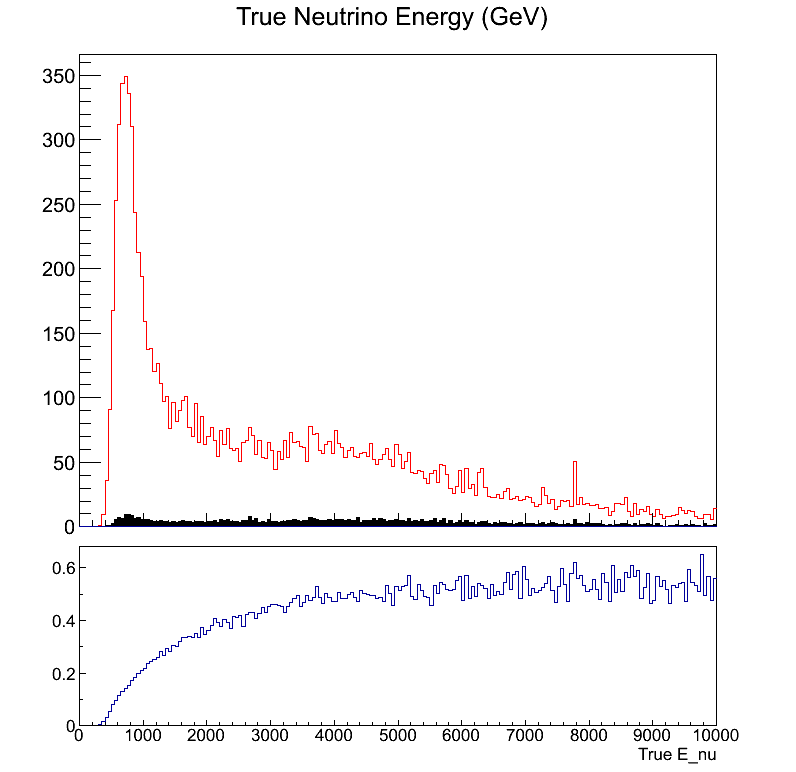
\includegraphics[width=2.5in]{Figures/TN100Plots/c_nuEair_3.png}
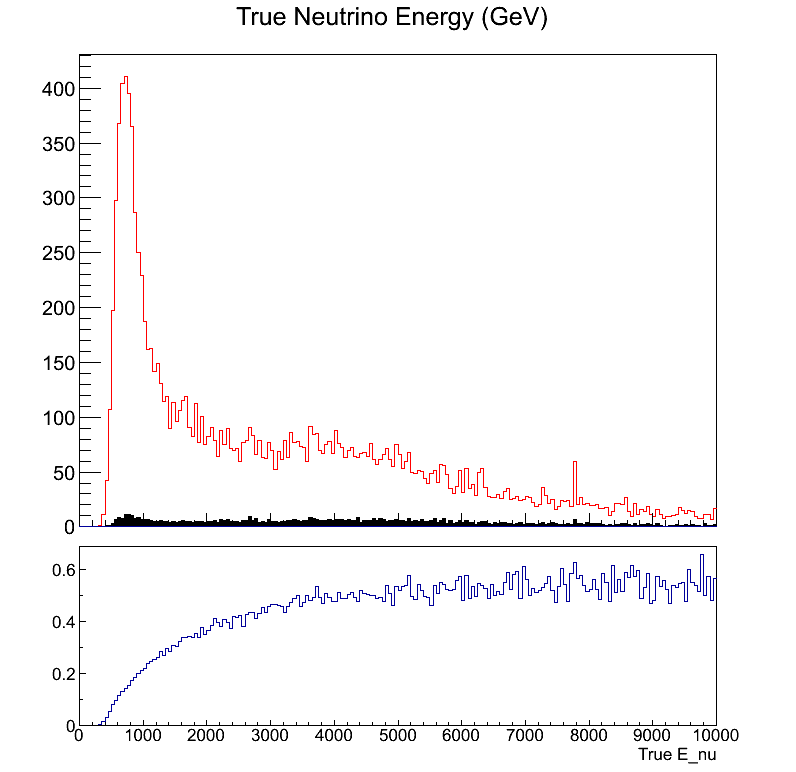
\includegraphics[width=2.5in]{Figures/TN100Plots/c_nuEair_4.png}
\caption{The true neutrino energy of selected events in NEUT MC. The red line shows the MC total selected events, the black fill shows the background events and the blue line shows the selection efficiency as a function of true neutrino energy. The top row of plots shows MC for water-in runs 1, 2 and 4 (left to right). The bottom row shows MC for water-out runs 2, 3 and 4 (left to right).}
\label{fig:nuEeff}
\end{figure}

\subsection{Cross Section Value}

Using the integrated flux, the known volume of water in the P0D, and the total expected signal events in each run period, we can use Formula \ref{eqn:xsec6} to evaluate the central value of the absolute water cross section. For 1902~kg of water, we have $1.145\times10^{30}$ nucleons. As this is the only target, we do not need to average out nucleus type. Using the flux term calculated in the previous section and the target number above, we measure an absolute water CC inclusive cross section of:

\begin{equation}
\left<\sigma\right>_\Phi = 6.51 \times 10^{-39} \frac{cm^2}{H_2O\:nucelon}.
\end{equation}

Note that this is only the central value before any corrections due to detector biases. We will deal with shifts in the central value of the cross section in the following section. Table \ref{tab:xscalc} shows the integrated flux per POT and calculated signal (N-B)/efficiency for each run that was used to measure the absolute, uncorrected, nominal cross section. The last column shows the nominal CC inclusive cross section calculated using an estimate of 5480~kg for the total mass in the P0D fiducial volume. The exact mass of the entire fiducial volume is not as well constrained as the mass of the water. We also show the water-in and water-out CC inclusive cross sections on the P0D as a combination of materials. Before applying any of the systematic corrections, we note that water-in and water-out cross sections are very similar. This happens as carbon, the primary material in the P0D, is known to have a similar cross section to water.

\begin{table}[h]
\caption{The total calculated signal (N-B)/eff and the integrated flux per POT for each run. These values are used to calculate the uncorrected nominal cross section on water. The last column also shows an uncorrected estimation of a CC inclusive cross section for all P0D materials combined.}
\centering
\begin{tabular}{cccc} \toprule
Run & (N-B)/e & Int. Flux ($10^{13}$~$\nu_\mu$/$10^{21}$ POT) & Cr. Sec. ($10^{-39}$cm$^2$/nucleon)\\
\hline
Run 1 water-in & 11698.2 & 1.9042 & 6.32\\ 
Run 2 water-in & 17811.7 & 1.92516 & 6.54\\ 
Run 2 water-out & 9263.16 & 1.92516 & 6.29\\ 
Run 3 water-out & 37518.9 & 1.92639 & 6.71\\ 
Run 4 water-in & 68044 & 1.93972 & 6.55\\ 
Run 4 water-out & 42593.7 & 1.93972 & 6.43\\ 
\hline
Water-in & 97554 & & 6.52\\
Water-out & 89376 & & 6.53\\
\hline
\bottomrule
\end{tabular} 
\label{tab:xscalc}
\end{table}